\section{Camera}
\label{sec:camera}
\subsection{Webcam}
\label{subsec:webcam}
A simple webcam is not enough to capture fast moving objects with sufficient quality. 
There are several reasons for this.
Firstly, certain parameters, such as the exposure time, cannot be adjusted by the user.
This would be necessary to capture the contours of the object being thrown as detailed as possible.
Secondly, conventional webcams work with a rolling shutter.
Technically this means that fewer sensors are used. Therefore, one sensor processes several pixels one after the other \cite{shuttermode}.

This results in the rolling shutter effect when the image changes.
On the one hand this effect is noticeable when the light flickers quickly.
For example the upper part of an image can be brighter than the lower part.
On the other hand there are problems with moving pictures.
The lower part of the image was taken at a later time, so the object appears distorted \cite{global_rolling_shutter}.

To eliminate this problem, some cameras feature the global shutter. 
This takes all pixels at the same time and stores them. 
Thus, no distortions in the image occur.

This can be shown well with an example.
In figure \ref{subfig:rollingshutter} is a recording of a ball with rolling shutter. 
Figure \ref{subfig:globalshutter} shows the same object, taken with a global shutter camera.
The distortion from the rolling shutter is clearly visible and deforms the effective object.

\begin{figure}[ht]
	\centering
	\begin{subfigure}[b]{0.4\textwidth}
		\centering
		
\includegraphics[width=0.3\textwidth]{rollingshutter}
		\caption{Rolling shutter}
		\label{subfig:rollingshutter}
	\end{subfigure}
	\begin{subfigure}[b]{0.4\textwidth}
		\centering
		
\includegraphics[width=0.3\textwidth]{globalshutter}
		\caption{Global shutter}
		\label{subfig:globalshutter}
	\end{subfigure}
	\caption{Difference rolling shutter and global shutter camera \cite{shuttermode}}
	\label{fig:shuttermode}
\end{figure}

\subsection{Baumer Industrial Camera}
\label{subsec:baumer_cam}

In addition to the global shutter requirement, the camera must also meet other specifications.

To ensure that an image is always received even from fast objects, the maximum duration between two images is

\begin{equation}
  T_\text{max} = \frac{f_\text{w} \cdot 0.75}{v_\text{max}} = \frac{\SI{0.69}{m} \cdot 0.75}{\SI{30}{\frac{m}{s}}} = \SI{17.25}{ms}.
  \label{eq:needed_T}
\end{equation}

It is assumed that the object is thrown in the last quarter of the booth and the maximum throwing speed is \SI[fraction=sfrac]{30}{\metre\per\second}.
This speed is approximately half the speed of the fastest baseball throw and is more or less attainable for an adult with the objects present \cite{speed_baseball}.

From equation \ref{eq:needed_T} it can be seen that the camera needs a frame rate which is higher than

\begin{equation}
  f_\text{min} = \frac{1}{T_\text{max}} = \frac{1}{\SI{17.25}{ms}} = \SI{58}{fps}.
  \label{eq:needed_fps}
\end{equation}

In order to capture the contours of the objects being thrown as detailed as possible, the motion blur must be kept to a minimum. 
This can be achieved by short exposure time. 
With the assumption that the motion blur should be smaller than or equal \SI{3}{cm}, there results a maximum exposure time of the camera of

\begin{equation}
  t_\text{exp} = \frac{s_\text{max}}{v_\text{max}} = \frac{\SI{0.03}{m}}{\SI{30}{\frac{m}{s}}} = \SI{1}{ms}.
  \label{eq:texp}
\end{equation}

In this project a VCXU-13C camera from Baumer is used.
The Baumer company produces various sensors, such as CMOS sensors with different specifications.
The VCXU-13C has global shutter.
Furthermore, it has a USB 3.0 interface for data transfer.
This is required because the Ultra96-V2 does not support an Ethernet interface.
The camera's frame rate is \SI{222}{fps}, which guarantees at least three pictures of each throw.
The minimum exposure time is \SI{20}{\micro s} \cite{baumer_cam}.

The camera requires a lens as well.
Suitable for the camera is the lens ZVL-FL-HC0614-2M, which is also manufactured by Baumer.
The aperture is manually operated to focus the images.

\subsection{Diffuse Lighting}
\label{subsec:Lighting}
The more light there is, the shorter the exposure time can be selected.
This results in a clearer image, which is an advantage in image recognition.
In order for the objects to be as independent of the lighting as possible, the lighting must not flicker and the field of view should be illuminated as uniformly as possible.

The SVL BAR LIGHT LHF300-WHI from Stemmer Imaging meets these requirements.
A completely uniformly illuminated image cannot be achieved with a single LED bar.
In the data sheet Stemmer specifies the illumination of a \SI{1}{m} $\times$ \SI{1}{m} image section according to graphic \ref{fig:lighting_LEDBAR}.
The distance from the camera to the measuring surface is \SI{0.5}{m}.
The green frame corresponds to the field of view.
The illumination is therefore very satisfying.

\begin{figure}[h]
	\centering
	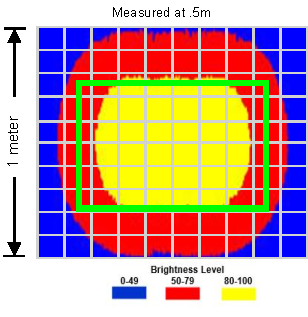
\includegraphics[width=0.3\textwidth]{graphics/brightness_level.pdf}
	\caption{Brightness Distribution according to Stemmer \cite{stemmer_datasheet}}
	\label{fig:lighting_LEDBAR}
\end{figure}